\subsection{Cross Sections as a function of the struck neutron momentum} 
%Results in \tkipn }
The momentum imbalance between the initial neutrino momentum and the sum of the final state lepton and hadron momenta.  In the limit of no intranuclear momentum transfer, it represents the momentum of the struck neutron (\tkipn).  This observable can be extracted using the following equation:
\begin{equation}
    \tkipn = \sqrt{\tkidelta^2 + \tkipl^2}
    \label{eq:pn}
\end{equation}
where \tkidelta\ is the net transverse momentum of the muon and proton system and \tkipl\ is defined in Equation \ref{eq:pl}. MINERvA has measured it before on scintillator in the LE run~\cite{MINERvA:2018hba}.  The peak at low \tkipn \ comes from events with little FSI and has a position and width reflecting the Fermi momentum of the struck neutron.  The tail at larger \tkipn \ largely comes from FSI processes that decelerate the proton and pion absorption. A smaller (larger) tail implies less (more) FSI. The differential cross section as a function of \tkipn \ for interactions on the CH, C, H$_{2}$O, Fe, and Pb targets, respectively, are shown in Fig.~\ref{figure:xsec_pn}. 
% tki_pn xsecs

\begin{figure}[h] 
	\centering
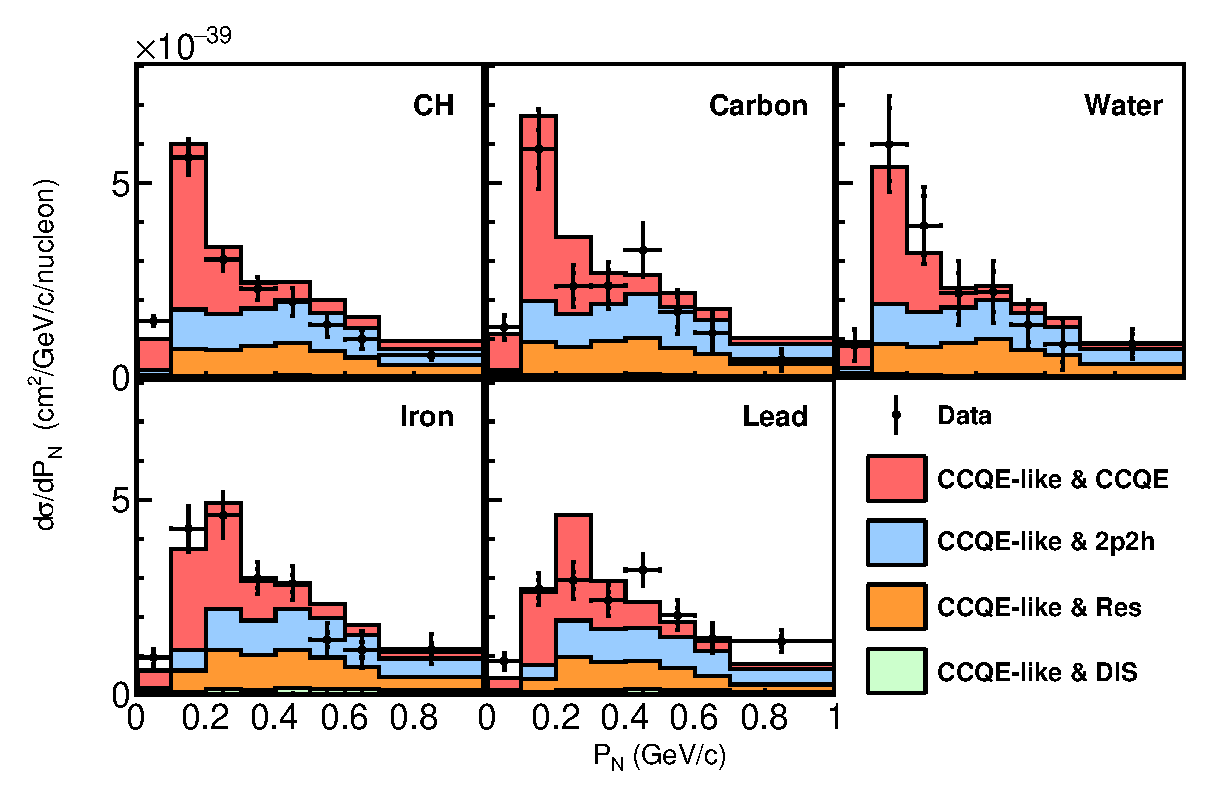
\includegraphics[width=\linewidth]{Figures/xsec_five_square/pn.eps}
	\caption{The differential cross section as a function of \tkipn\ for CH, C, H$_{2}$O, Fe, and Pb targets, along with the predictions for the different quasielastic-like signal processes.}
	\label{figure:xsec_pn}
\end{figure}

The MINERvA tune qualitatively describes the data fairly well for the smaller nuclei.   It also follows the data with the reduction of the no-FSI peak and enhancement of the FSI-induced tail with increasing $A$.  The uncertainties broken down by source for both the absolute cross sections and the cross section ratios as a function of \tkipl\ can be found in Fig.~\ref{fig:xsec_err_pl}.

The differential cross section as a function of \tkipn \ for the different targets as compared to a range of models is given in Fig.~\ref{fig:models_pn}. In this comparison, NEUT and the hN versions of GENIE predict substantially more cross section in the decelerating FSI in the tail than seen in the data, particularly for the larger nuclear targets.  NuWro tends to have more events in the low-side tail indicating more acceleration of the proton than seen in the data.  GiBUU and the hA verstions of GENIE do a fairly good job describing the data in this variable. The \chisq\ between the cross sections and the models can be found in Table~\ref{tab:neutronmomentum}.
% comparisons to generators p_n
\begin{figure}
    \centering 
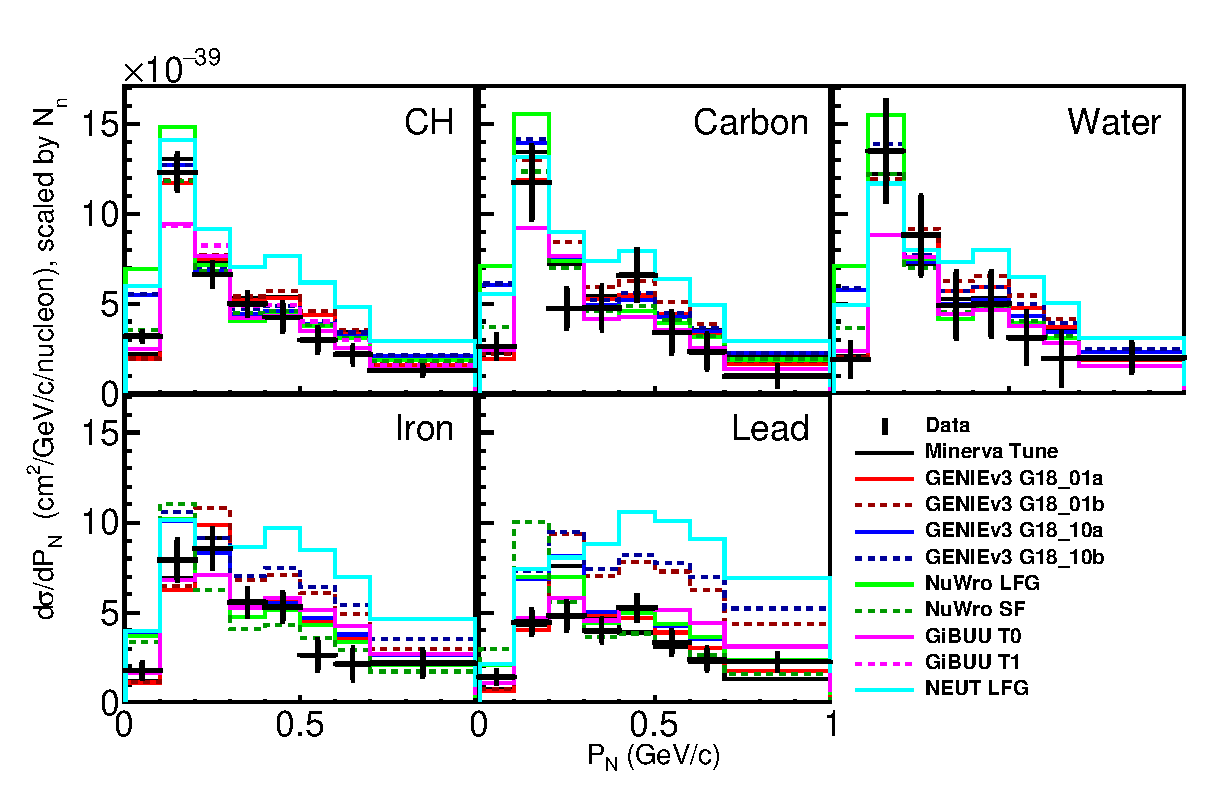
\includegraphics[width=\linewidth]{Figures/gencompare/pn_5square.eps}
    \caption{Cross section measurements and predictions as a function of \tkipn\ for different targets and for a selection of different generator and model choices.}
    \label{fig:models_pn}
\end{figure}
The ratio of the differential cross section as a function of  \tkipn \ for each nuclear target (C, H$_{2}$O, Fe, Pb) to that for scintillator is shown in 
Fig.~\ref{Figure:Gencompare_pn_ratio}. The models agree with the data well for the smaller targets.  For the Fe and Pb targets, the model spread is large.  NuWro SF has a much larger contribution to the ratio at low \tkipn \ than the data or any of the other models.  At higher \tkipn \ in the larger targets, NEUT and the GENIE hN  models tend to be higher than the data and the GENIE hA models and NuWro SF are lower than the data.  For interactions on Pb, the cross section ratio data disagree with the MINERvA Tune especially above \tkipn\ above 0.5~GeV.  This could be evidence for additional decelerating FSI in the tail and FSI processes that accelerate the proton on the low side of the \tkipn \ peak.  The \chisq\ between the cross sections and the models can be found in Table~\ref{tab:neutronmomentum}.
\begin{figure}
    \centering
                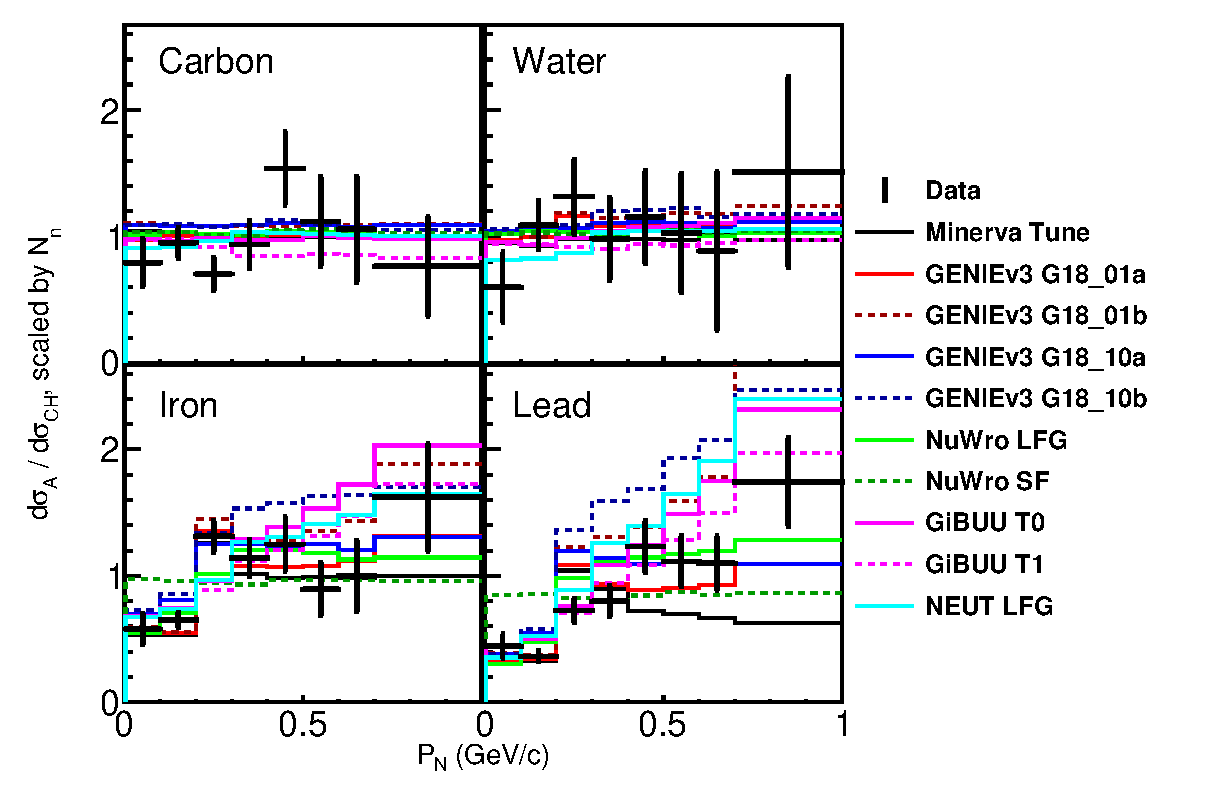
\includegraphics[width=\linewidth]{Figures/gencompare/pn_4square.eps}

    \caption{\tkipn\ cross-section ratio generator comparison for multiple targets.  Changes to the FSI model (GENIE ``a'' to ``b'') in GENIE change the cross section ratio most dramatically at high \tkipn\, and those changes are  larger than changes to the 2p2h model (GiBUU T0 to GiBUU T1) or changes to the initial state (GENIE 1 to GENIE 10) or (NuWro LFG to NuWro SF).}
        \label{Figure:Gencompare_pn_ratio}
\end{figure}
